\Chapter{A lekérdezőnyelv}

\section{Az adatbázis szerkezete}

A lekérdezőnyelv bemutatása előtt érdemes megnézni, hogy az adatbázis hogyan épül fel, és a nyelv egyes funkciói milyen gyakorlati problémákat oldanak meg. Ehhez a következő fogalmak tisztázására van szükségünk.
\begin{itemize}
\item \textit{adatbázis}: Az adatbázis a kezelendő adatok legnagyobb logikai egységét jelenti. Ez tartalmaz térképeket, osztálydefiníciókat.
\item \textit{térkép}: Az objektum példányok adatbázishoz kötődnek.
\item \textit{osztály}: A tárolandó elemek szerkezetét (\textit{sémáját}) írják le az osztálydefiníciók. Az alaptípusok esetében azokat az adatbázis közvetlenül biztosítja. Osztályokat a felhasználók is definiálhatnak, amelyeket azt követően az alaptípusokhoz hasonlóan tudnak majd használni.
\item \textit{objektum}: Az osztályokból objektumokat példányosíthatunk, ha megadjuk az e\-gyes attribútumok értékeit. Ezek az objektum példányok az adott térképhez kötődnek.
\item \textit{réteg}: A térképeknek van egy saját, lazább logikai felbontása, amely az objektumok egy diszjunkt csoportosítását adja. Azon objektumok, amelyek rendelkeznek pozícióval tartalmaznak még egy réteg azonosítót.
\item \textit{entitás}: Egy \texttt{Entity} alaptípusból létrehozott példány. Ezek azok, amelyek a térképen ténylegesen meg is fognak jelenni.
\end{itemize}

A következő szakaszok arra térnek ki, hogy a gyakorlatban előforduló gyakori problémákat milyen formában oldhatjuk meg a lekérdezőnyelv segítségével majd.

\subsection{Alkalmazáslogika kezelése}

Az adatbázisban tárolt elemekhez gyakran szükség lehet olyan további metaadatok megadására, amely az alkalmazáslogika kialakítása szempontjából lesz majd fontos. Ezeket a többletinformációkat saját osztályok definiálásával tudjuk megadni. Ez nagyon hasonló az SQL-ben a táblák sémájának definiálásához. Osztályok definiálási módjára a \texttt{CREATE} kifejezés bemutatásánál láthatunk majd példákat.

\subsection{Rétegkezelés}

Az adatbázis egy térképen belül rétegeket is értelmez. A térképek eredendően kétdimenziósak, ezzel viszont egy diszkrét, harmadik dimenziót is kapunk. Ez akkor lehet hasznos, amikor például ütközés vizsgálatnál a különböző szinteken lévő elemek ütközését külön-külön szeretnénk vizsgálni.

Két alapértelmezett attribútumot bevezetése volt szükség, úgy mint
\begin{itemize}
\item \texttt{zlayer}: A réteg azonosítószáma.
\item \texttt{zindex}: A rétegen belül egy sorszám, amely egyedi az objektumra nézve a rétegen belül.
\end{itemize}

A réteg és az index tehát az objektumot egyértelműen azonosítja. Ami miatt mégis szükség van az \texttt{id} azonosítóra, mert a réteg és az index is változtatható, ami egy azonosítónál nem szerencsés, illetve vannak nem réteghez kötött objektumok is.

Ha két elem más szinten van, akkor a \texttt{zlayer} attribútumuk értéke eltérő. Különböző rétegekben lévő objektumok között az ütközésvizsgálat nincs értelmezve.

A \texttt{zindex} attribútum megjelenítésnél a kirajzolási sorrend miatt érdekes. Mivel a rétegen belül nincs más sorrendi megkötés, ezért a takarási feladat csak így oldható meg.

Összefoglalva tehát minden objektumnak van \texttt{id}, \texttt{className}, \texttt{zlayer} és \texttt{zindex}.

\subsection{Térkép mentése és visszaállítása}

Az alkalmazások tipikusan a futtatások között is tárolják az adatokat. Az adatbázis használatának egyik nagy előnye, hogy így a program megírásánál a perzisztenciával már nem kell foglalkozni, mivel azt az adatbázis meg tudja oldani. Térképeket egyszerűen létre tudunk hozni, el tudjuk menteni benne az adatokat, illetve vissza tudjuk azokat tölteni.

\section{Alaptípusok}

A lekérdezőnyelv típusos. Tartalmaz előre definiált típusokat (\textit{alaptípusok}, \textit{gyári típusok}), illetve a nyelv lehetőséget ad új típusok definiálására is (\textit{felhasználói típusok}).

Az alaptípusok hierarchiáját \aref{fig:types} ábrán láthatjuk. Az élek itt tartalmazási kapcsolatot jelölnek. A nyelv csak kompozícióra ad lehetőséget.

A típusokból hasonlóképpen tudunk példányokat létrehozni, mint ahogy az objektum orientált programozási nyelvekben. A típus nevét követő zárójelekben adhatjuk meg a példány létrehozásához szükséges értékeket egy vesszővel elválasztott listában.

Minden objektumnak a típusa mellett van azonosítója is. Ezt az \texttt{id} attribútumában tárolja. Értéket példányosításkor automatikusan kap. Az objektumtól le tudjuk azt kérdezni, viszont változtatni nem lehet.

A következő szakaszokban az alaptípusok bemutatására kerül sor. A használati módjuk, paraméterezésük szemléltetéséhez már itt is lekérdezések szerepelnek, viszont azok részletes bemutatása majd csak a műveleti rész taglalásánál szerepel.

\begin{figure}[htb]
\begin{center}
    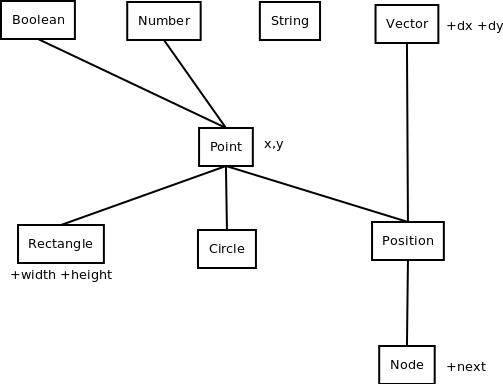
\includegraphics[scale=0.5]{images/types}
    \caption{A lekérdezőnyelv alaptípusai}
    \label{fig:types}
\end{center}
\end{figure}

\subsection{Boolean}

A \textit{Boolean} a nyelvben a logikai adattípus. Értéke \texttt{true} vagy \texttt{false} lehet. Paraméter nélküli létrehozás esetén az alapértelmezett értéke \texttt{false}. Az alábbi példákban az \texttt{azeroth} nevű térképre kerülnek beszúrásra logikai értékek.

\begin{sql}
INSERT Boolean() INTO azeroth;
INSERT Boolean(true) INTO azeroth; 
INSERT Boolean(false) INTO azeroth;
INSERT Boolean(
    SELECT bool FROM azeroth
    WHERE bool IS Boolean AND bool.id = "bool11"
) INTO azeroth;
\end{sql}

Az utolsó példából látható, hogy a logikai típusú objektum is teljes értékű objektum, így az is rendelkezik azonosítóval (\texttt{id}).

\subsection{Number}

A \textit{Number} típus valós vagy egész szám 4 byteon való tárolására alkalmas. A lekérdezőnyelv nem különböztet meg előjeles és előjel nélküli változatot.

\begin{sql}
INSERT Number(1.2) INTO azeroth;
INSERT Number(12) INTO azeroth;
INSERT Number(
    SELECT number FROM azeroth
    WHERE number IS Number AND number.id = "numberasd11"
) INTO azeroth;
INSERT Number(
    SELECT number FROM azeroth
    WHERE number HAS x AND number.x IS Number AND number.id = "num11"
) INTO azeroth;
\end{sql}

\subsection{String}

Szöveges értékek tárolására a \textit{String} típust használhatjuk.

\begin{sql}
INSERT String("alma") INTO azeroth;
INSERT String(
    SELECT string FROM azeroth
    WHERE string IS String AND string.id = "stringasd11"
)
INTO azeroth;
\end{sql}

\subsection{Point}

A térképen az elemek helyét pontok adják, amelyet \textit{Point} típusú objektumokban tárolhatunk. A pontnak sem kiterjedése, sem iránya nincs. Tulajdonképpen két \textit{Number} típusú értéket fog össze egy egységbe. A pont koordinátáit a geometriában használatos $(x, y)$ párral adhatjuk meg.

\begin{sql}
INSERT Point(10, 20) INTO azeroth;
INSERT Point(Number(10), Number(20)) INTO azeroth;
INSERT Point(Number(10), 20) INTO azeroth;
INSERT Point(10, Number(20)) INTO azeroth;
INSERT Point(Point(10, 10)) INTO azeroth;
INSERT Point(
    SELECT point FROM azeroth
    WHERE point IS Point AND point.id = "pointasd11"
) INTO azeroth;
\end{sql}

Az utolsó beszúrás esetében egy másik \textit{Point} típusú objektumra hivatkozunk.

\noindent Amennyiben annak az értéke változik valamelyik a kettő közül, akkor ennek is változni fog.

\begin{sql}
INSERT Point(
    SELECT number FROM azeroth
    WHERE number is Number AND number.id = "numasd11", 10
) INTO azeroth;
\end{sql}

Ilyenkor a pont \texttt{x} attribútuma egy másik \textit{Number} típusú objektumra mutat, tehát ha az változik, akkor a pont attribútuma is fog.

\begin{sql}
INSERT Point(
    SELECT number FROM azeroth
    WHERE number is Number AND number.id = "numasd11",
    SELECT number FROM azeroth
    WHERE number is Number AND number.id = "numasd12"
) INTO azeroth;
\end{sql}

Ebben mind a két attribútuma más \textit{Number} objektumra mutat.

\subsection{Vector}

A \textit{Vector} típus itt a geometriai értelemben véve irány tárolását teszi lehetővé. A ponthoz hasonlóan ez is két \textit{Number} értéket fog össze, ennek viszont csak iránya van, helye nincsen.

\begin{sql}
INSERT Vector(10, 20) INTO azeroth;
INSERT Vector(Number(10), Number(20)) INTO azeroth;
INSERT Vector(Number(10), 20) INTO azeroth;
INSERT Vector(10, Number(20)) INTO azeroth;
INSERT Vector(Vector(10, 20)) INTO azeroth;
INSERT Vector(
    SELECT vector FROM azeroth
    WHERE vector IS Vector AND vector.id = "vetorasd11"
) INTO azeroth;
\end{sql}

Ilyenkor egy másik \textit{Vector} objektumra hivatkozik, tehát ha annak az értéke változik valamelyik a kettő közül, akkor ennek is fog.

\begin{sql}
INSERT Vector(
    SELECT number FROM azeroth
    WHERE number is Number AND number.id = "numasd11", 10
) INTO azeroth;
\end{sql}

Ilyenkor a vector \texttt{dx} attribútuma egy másik \textit{Number} objektumra mutat, tehát ha az változik, akkor ez is fog.

\begin{sql}
INSERT Vector(
    SELECT number FROM azeroth
    WHERE number is Number AND number.id = "numasd11",
    SELECT number FROM azeroth
    WHERE number is Number AND number.id = "numasd12"
) INTO azeroth;
\end{sql}

A ponthoz hasonlóan itt is megadható függetlenül a két \textit{Number} érték.

\subsection{Dimension}

Egy szélesség és egy magasság értéket tárol. Mindkettő típusa \textit{Number}.

\begin{sql}
INSERT Dimension(10, 20) INTO azeroth;
INSERT Dimension(Number(10), Number(20)) INTO azeroth;
INSERT Dimension(Number(10), 20) INTO azeroth;
INSERT Dimension(10, Number(20)) INTO azeroth;
INSERT Dimension(Dimension(10,10)) INTO azeroth;
INSERT Dimension(
    SELECT dimension FROM azeroth
    WHERE dimension IS Dimension AND dimension.id="dimensionasd11"
) INTO azeroth;
\end{sql}

Az utóbbi esetben egy másik Dimension objektumra hivatkozik, tehát ha annak az értéke változik valamelyik a kettő közül, akkor ennek is fog. Hasonlóan kezelhetjük az egyes esetek külön-külön hivatkozásokkal való megadását is, mint ahogy a pont és a vektor esetében.

\begin{sql}
INSERT Dimension(
    SELECT number FROM azeroth
    WHERE number is Number AND number.id = "numasd11", 10
) INTO azeroth;
INSERT Dimension(
    SELECT number FROM azeroth
    WHERE number is Number AND number.id = "numasd11",
    SELECT number FROM azeroth
    WHERE number is Number AND number.id = "numasd12"
) INTO azeroth;
\end{sql}

Az utolsóban szintén itt is mind a két attribútuma más \textit{Number} típusú objektumra mutat.

\subsection{Rectangle}

A \textit{Rectangle} típus téglalap adatainak tárolására szolgál. Tartalmaz egy pontot, amelyben tárolja a bal felső sarkának koordinátáit, illetve egy kiterjedést, amely a szélesség és magasság attribútumokat adja.

\begin{sql}
INSERT Rectangle(Point(10,10), Dimension(100, 200)) INTO azeroth;
INSERT Rectangle(Rectangle(10, 10, 100, 100)) INTO azeroth;
\end{sql}

Itt az a lényeg, hogy lehet belül azzal a new nélküli kifejezéssel is visszaadatni új objektumot.

\begin{sql}
INSERT Rectangle(10, 10, 100, 200) INTO azeroth;
INSERT Rectangle(10, 10, Dimension(100, 200)) INTO azeroth;
INSERT Rectangle(Point(10, 10), 100, 200) INTO azeroth;
INSERT Rectangle(
    SELECT rectangle FROM azeroth
    WHERE rectangle IS Rectangle AND id = "rectasd11"
) INTO azeroth;
INSERT Rectangle(
    SELECT number FROM azeroth
    WHERE number is Number AND number.id = "numasd11",
    SELECT number FROM azeroth
    WHERE number is Number AND number.id = "numasd12",
    SELECT number FROM azeroth
    WHERE number is Number AND number.id = "numasd13",
    SELECT number FROM azeroth
    WHERE number is Number AND number.id = "numasd14"
) INTO azeroth;
\end{sql}

Itt mind a 4 paraméter egy lekérdezés eredménye, azaz mind mutat egy másik objektumra.
Attól függetlenül, hogy hozzuk létre a téglalapot, ezeket egy pont és egy kiterjedés objektumban fogja tárolni.

\subsection{Oval}

Az \textit{Oval} típus ovális alakzatok tárolását teszi lehetővé. 

\begin{sql}
INSERT Oval(x, y, width, height) INTO azeroth 
VALUES(10, 300, 12, 32);
\end{sql}

A fenti lekérdezés eredménye, hogy egy olyan oválist illeszt az "azeroth" nevű térképre, aminek a bal felső befoglaló téglalapjának a sarka a $(10, 300)$ pontra esik, a szélessége 12, a magassága 32. 

\subsection{Position}

A pozíciók leírásához használhatjuk a \textit{Position} osztályt. Ennek van helye és iránya. Lényegében egy pont és egy vektor objektumot fog össze egy logikai egységbe.

\begin{sql}
INSERT Position(Point(10, 10), Vector(100, 100)) INTO azeroth;
INSERT Position(Position(10, 10, 100, 100)) INTO azeroth;
\end{sql}

A pozíciókat közvetlenül az attribútumok értékeivel, vagy pedig részlegesen a részobjektumaival is példányosíthatjuk.

\begin{sql}
INSERT Position(10, 10, 100, 200) INTO azeroth;
\end{sql}

Ebben az esetben a sorrend \texttt{x}, \texttt{y}, \texttt{dx} és \texttt{dy}. 

\begin{sql}
INSERT Position(10, 10, Vector(100, 200)) INTO azeroth;
INSERT Position(Point(10, 10), 100, 200) INTO azeroth;
INSERT Position(
    SELECT position FROM azeroth
    WHERE position IS Position AND id = "posasd11"
) INTO azeroth;
INSERT Rectangle(
    SELECT number FROM azeroth
    WHERE number is Number AND number.id = "numasd11",
    SELECT number FROM azeroth
    WHERE number is Number AND number.id = "numasd12",
    SELECT number FROM azeroth
    WHERE number is Number AND number.id = "numasd13",
    SELECT number FROM azeroth
    WHERE number is Number AND number.id = "numasd14"
) INTO azeroth;
\end{sql}

Ezekben is, az előzőekhez hasonlóan objektum hivatkozások jönnek létre a példányosítás során.

\subsection{Node}

A nyelv a dinamikus adatszerkezetek leírását láncolással oldja meg. Az alkalmazási területeket figyelembe véve általában pozíciók láncolására lehet szükség. A \textit{Node} típus egy pozíció típusú attribútumot és egy hivatkozást tartalmaz a következő \textit{Node} objektumra. Ennek a segítségével megadhatunk útvonalakat, fákat vagy általános irányított gráfokat.

\begin{sql}
INSERT Node(Node(10, 10, 100, 100, NULL)) INTO azeroth;
\end{sql}

A csomópontnak ekkor a pozícióra jellemző attribútumait egészítjük ki egy referenciával. A \texttt{NULL} ez esetben a sehova sem mutató, érvénytelen referenciát jelenti.

\begin{comment}{Egységesen kellene a true, false-al!}
\end{comment}

\begin{sql}
INSERT Node(10, 10, 100, 100, NULL) INTO azeroth;
INSERT Node(10, 10, 100, 100,
    SELECT node FROM azeroth
    WHERE node IS Node AND node.id = "nodeasd11"
) INTO azeroth;
\end{sql}

Itt már úgy hozunk létre egy csomópontot, hogy az egy másik, már létező csomópontra mutat.

\begin{sql}
INSERT Node(10, 10, 100, 100, Node(200, 200, 2000, 2000, NULL))
INTO azeroth;
\end{sql}

A nyelv ezt a megoldást is lehetővé teszi. Ilyenkor a belső csomópont objektumra fog mutatni, ami viszont ilyenkor még nincs a térképen, de ez így egyúttal létre is hozza, hogy ő hivatkozik rá a láncban.

\begin{sql}
INSERT Node(10, 10, 100, 100, NULL, true) INTO azeroth;
\end{sql}

Ha az 5. paraméternek egy \texttt{true} értéket adunk meg, akkor az azt jelenti, hogy ez egy Lánc első eleme, innen indul ki az összes többi. (Amennyiben az utolsó elem erre mutat, akkor kapunk egy körutat.)

\begin{sql}
INSERT Node(10,10, 100, 100, NULL, false) INTO azeroth;
\end{sql}

Így is létrehozható egy csomópont. Ez az alapértelmezett eset, tehát ha nem tüntetjük fel, hogy az utolsó paraméter értéke \texttt{false}, akkor alapértelmezés szerint ugyanezt kapjuk.

\begin{comment}{Ennek az utolsó paraméternek majd még utána kell gondolni!}
\end{comment}

\begin{sql}
INSERT Node(10,10, 100, 100) INTO azeroth;
\end{sql}
Ha elhagyjuk azt a paramétert, ami a következő csomópontra mutatna, akkor azzal sincs semmi gond, mert az automatikusan beilleszti oda a NULL értéket.

\subsection{Path}

A \textit{Path}, útvonal típus csomópontok halmazát tárolja.

\begin{sql}
INSERT Path(
    Node(10,10,10,10),
    Node(10,20),
    Node(10,10,100,35)
) INTO azeroth;
\end{sql}

Itt az útvonal úgy jön létre, hogy a paraméterlistában szereplő csomópontokat úgy hozza létre, hogy paraméterlistában való elhelyezkedés szerint adja értékül a \texttt{next} értéknek mindig a következőt. Az utolsó elem \texttt{next} attribútuma \texttt{NULL} értéket kap.

Minden csomópont objektumnak van egy \texttt{isFirst} logikai típusú attribútuma, ami csak az első elemnek vesz fel igaz értéket, hogy tudjuk honnan indul az útvonal. Ez az \texttt{isFirst} az útvonal létrehozási mechanizmusban automatikusan kap értéket, erről a felhasználónak nem kell gondoskodnia.

Látható, hogy az egyik csomópontot kevesebb (mindössze kettő paraméterrel) hoztuk létre. Ez nem jelent semmi problémát, ilyenkor az irány nincs megadva, de arra nem is feltétlenül van szükség.

A \textit{Node} adattípus leírásánál elmondtuk, hogy a \texttt{Node(10, 10, 10, 10)} hívással nem adjuk meg a következő Nodera mutató elemet, így az autómatikusan NULL lesz. Amennyiben ez  \textit{Path} inicializálásnál történik, akkor a következő csomópont hivatkozását kapja meg (amennyiben nem az utolsó helyen szerepel a paraméter).

\begin{sql}
INSERT Path(
    SELECT node FROM azeroth
    WHERE node IS Node AND node.id = "nodeasd11"
) INTO azeroth;
\end{sql}

Egy útvonal nem hozható létre a meglévő csomópontok összegyűjtéséből. Az útvonal inicializálásnál nem szerepelhet egyetlen szelekciós utasítás sem, mert az hibákhoz vezetne.

Egy objektum ha referenciát tartalmaz egy másik objektumra akkor az eléri bármikor a hivatkozottat, viszont a hivatkozott nem tud hivatkozni arra aki rá hivatkozik. Erre nincs nyelvi elem definiálva, hisz a gyakorlatban ritkán van erre szükség, kevés esetben lenne alkalmazható, így kimaradt a lekérdező nyelv eszközkészletéből.

\section{Logikai operátorok}

\begin{sql}
=  <=  >=  >  <  <>
OR  AND  NOT  IS  COLLIDE
\end{sql}

A fenti operátorok logikai operátorok, tehát \texttt{Boolean} típusú értékkel térnek vissza.

Lássunk mindegyikre egy példát!

\begin{sql}
SELECT mine FROM azeroth WHERE mine.id = "asd11";
SELECT mine FROM azeroth WHERE mine.x <= 10;
SELECT mine FROM azeroth WHERE mine.y >= 10;
SELECT mine FROM azeroth WHERE mine.x <> 20;
\end{sql}

A \texttt{mine.x} operandus a háttérben egy \texttt{mine HAS x} feltételt is jelent, de ezt nem kell feltüntetnie a felhasználónak. A \texttt{mine HAS x} jelentése, hogy az adott objektumnak van x attribútuma, vagy sem. Sokáig nyelvi szinten megtalálható volt a \texttt{HAS} operátor, viszont a kényelmi szempontok miatt ezt implicit módon tartalmazzák mostmár az említett nyelvi szerkezetek.
 
\begin{sql}
SELECT mine FROM azeroth WHERE mine.stone.location.x > 10;
\end{sql}

A fent látható lekérdezés olyan objektumokat kérdez le, amelyeknek van \texttt{stone} attribútuma, aminek van \texttt{location} attribútuma, aminek van \texttt{x} attribútuma. Ezekre a \texttt{HAS} feltétel kiértékelődik, illetve további feltételként az, hogy az \texttt{x} attribútumnak értéke nagyobb mint 10.

\begin{sql}
SELECT mine FROM azeroth WHERE mine IS Mine;
\end{sql}

Az \texttt{IS} operátor az objektum típusának ellenőrzésére szolgál, az \texttt{IS} bal oldalán egy szimbólum, jobb oldalán pedig egy osztálynév kell szerepeljen.

\begin{sql}
SELECT mine FROM azeroth WHERE mine.x = 10 AND mine.y < 20;
\end{sql}

A logikai műveletek a \texttt{WHERE} után kombinálhatóak is természetesen:

\begin{sql}
SELECT mine FROM azeroth
WHERE mine.x = 10 AND mine.y = 20 OR mine.id = 100;
\end{sql}

Ha nincs zárójelezés, akkor sorban veszi a feltételeket.

\begin{sql}
SELECT mine FROM azeroth
WHERE mine.x = 10 AND (mine.y = 20 OR mine.id = 100);
\end{sql}

\begin{sql}
SELECT mine FROM azeroth
WHERE mine.x = 10 AND NOT (mine.y = 20 OR mine.id = 100 OR 10 = 10);
\end{sql}

A fenti lekérdezés azokat az objektumokat gyűjti ki, amelyek \texttt{x} attribútuma 10, és \texttt{y} attribútuma nem egyenlő 20, és az azonosítójuk nem egyenlő 100-al.

Az alábbi lekérdezés azokat az objektumokat választja ki, amelyek nem tartalmazzák a $(10, 10)$ pontot.
\begin{sql}
SELECT mine FROM azeroth
WHERE NOT(mine COLLIDE POINT(10, 10));
\end{sql}


A kiértékelésben a zárójelnek szerepe lehet, ezt az eszközt a felhasználó kezébe adja az adatbázis.

\section{Metódusok}

Csak a nyelv alaptípusai (\texttt{Boolean}, \texttt{Number}, \texttt{Vector}, \texttt{Rectangle}, stb.) rendelkeznek metódusokkal. Amikor a felhasználó készít saját osztálydefiníciót, ő csak adatleírást végezhet, metódusokat nem definiálhat hozzájuk. Az alaptípusokhoz elkészített metódusok a típusokhoz valamely szolgáltatást jelentenek. Jelenleg egyetlen metódust definiáltunk a lekérdezőnyelvbe, amely a \texttt{distanceFrom(Number x, Number x)}. Ez a metódus visszaad egy \texttt{Number} értéket, amely a távolság az objektum és a megadott pont között. Ezt a metódust minden olyan objektumra meg lehet hívni, amely rendelkezik $(x, y)$ koordinátákkal, illetve szélesség (\texttt{width}), és magasság (\texttt{height}) attribútumokkal.

\section{DDL adatdefiníciós utasítások}

\subsection{Adatbázisok és térképek létrehozása}

Adatbázist, benne térképeket és osztályokat egyaránt a \texttt{CREATE} lekérdezéssel lehet létrehozni.

A \texttt{db} nevű adatbázist például a
\begin{sql}
CREATE DATABASE db;
\end{sql}
lekérdezéssel tudjuk létrehozni. Az adatbázis fogja össze a benne tárolt térképeket. 

Térképet létrehozni hasonlóképpen a
\begin{sql}
CREATE MAP azeroth;
\end{sql}
formában lehet. Ekkor az aktuálisan megnyitott adatbázison belül jön létre egy \texttt{azeroth} nevű térkép.

\subsection{Saját osztályok definiálása}

Osztályt definiálni például az alábbi formában lehet.
\begin{sql}
CREATE CLASS Mine(
    Number age,
    String name,
    Number x,
    Number y
); 
\end{sql}
Automatikusan minden \texttt{INSERT} lekérdezés hatására beillesztődik egy \texttt{id} attribútum az objektumhoz. A definiált osztályok ezt implicit tartalmazzák, azt nem kell definiálni a \texttt{CREATE} lekérdezésben.

Amikor definiálunk egy osztályt, akkor nincs lehetőségünk származtatásra. Tervezéskor a kompozíciót tartottuk a megfelelő megoldásnak, ami azt jelenti, hogy nem leszármaztatunk egy osztályból, hanem adattagként tároljuk azt, és tovább hívjuk annak metódusait.

Az osztálydefiníciókban természetesen megadhatunk attribútum típusként más osztálydefiníciókat is, például:
\begin{sql}
CREATE CLASS Mine(
    Stone stone,
    Number size
);

CREATE CLASS Mine(
	Number kor DEAFAULT 18
);
\end{sql}

A \texttt{DEFAULT} integritási feltétel azt jelenti amit az SQL nyelvben, tehát, ha az adott attribútum \texttt{INSERT} lekérdezés hatására nem töltődik fel, akkor a \texttt{DEFAULT} kulcsszó után feltüntetett érték fog automatikusan adódni neki. \texttt{DEFAULT} csak primitív típusú attribútumoknál használható.

A térképeket és osztályokat is az adatbázis fogja össze. Amikor létrehozunk egy osztálydefiníciót, akkor azt az adatbázishoz definiáljuk, nem pedig külön a térképekhez, tehát az azonos adatbázisban tárolt térképeken azonos típusú objektumokat tárolhatunk.

Az objektum azonosítók automatikus kiosztása úgy történik, hogy minden térképen külön számláló van erre a célra. Emiatt két térképen is lehet azonos azonosítójú elem. Az azonosítók tehát térképre nézve lokálisak, a térképek elemei így nem keveredhetnek.

\subsection{Adatbázis, térkép és osztályok törlése}

Egy adatbázist, térképet és osztálydefiníciót a \texttt{DROP} lekérdezéssel lehet, például:
\begin{sql}
DROP DATABASE db1;
DROP MAP azeroth;
\end{sql}
A két fenti utasítás értelemszerűen törlést visz végbe. Ha törlök egy adatbázist, akkor minden benne lévő térkép és osztálydefiníció törlődik.

Osztálydefiníció törölni, például
\begin{sql}
DROP CLASS Mine;
\end{sql}
csak akkor lehet, ha egyik térképen sem tartozik már hozzá létrehozott példány.

\subsection{Osztálydefiníciók megváltoztatása}

Az adatbázis szerkezetét az \texttt{ALTER} lekérdezéssel lehet megváltoztatni. Ez elsősorban az osztálydefiníciók módosítását jelenti. Ahogy a törlésnél, a szerkezet megváltoztatása itt is csak akkor lehetséges, ha az adott osztálydefinícióhoz nem tartozik példány.

\begin{comment}{Ez így nem túl erős megkötés?}
\end{comment}

A lekérdezésnek 4 altípusa van.
\begin{itemize}
\item
Az \texttt{ADDATTRIBUTE} utasítással meglévő osztályhoz adhatunk hozzá egy újabb attribútumot, például
\begin{sql}
ALTER CLASS Mine ADDATTRIBUTE name String;
\end{sql}
\item
A \texttt{RENAMEATTRIBUTE} utasítással egy meglévő attribútumot nevezhetünk át a \texttt{TO} kulcsszó után szereplő értékre. Innentől kezdve ezen a néven lehet rá hivatkozni. Ilyen lekérdezés például az
\begin{sql}
ALTER CLASS Mine RENAMEATTRIBUTE size TO name;
\end{sql}
\item
Attribútumot eltávolítani a \texttt{DELETEATTRIBUTE} kulcsszóval lehet. Például a \texttt{size} attribútumát a \texttt{Mine} osztálydefiníciónak az alábbi lekérdezéssel lehet törölni
\begin{sql}
ALTER CLASS Mine DELETEATTRIBUTE size;
\end{sql}
\item
A RENAMECLASS az osztály nevének megváltoztatása szolgál, például
\begin{sql}
ALTER CLASS Mine RENAMECLASS BigMine;
\end{sql}
\end{itemize}

\section{DML adatkezelő utasítások}

\subsection{Objektumok létrehozása}

Új objektum felvinni egy térképre \texttt{INSERT} lekérdezéssel lehet, például
\begin{sql}
INSERT Szobor(location, name) INTO azeroth
VALUES((10, 10), "Jani") LAYER 1;
\end{sql}
A \texttt{LAYER 1} azt jelenti, hogy a beszúrandó elemek az 1-es rétegre kerüljenek, tehát a \texttt{zlayer} attribútumát 1-re kell állítani, a \texttt{zindexet} pedig az 1-es rétegben lévő következő indexre. Mivel rétegből tetszőleges sok lehet, ezért a kiosztandó indexek rétegenként egyediek.

Az alábbi lekérdezés már az összetettebbek közé tartozik. Szükséges megadni az osztálynév után a attribútumok felépítését. Ezzel mondjuk meg, hogy mely atribútumok kapnak értéket a \texttt{VALUES} kulcsszó után felsorolt értékhalmazból.
\begin{sql}
INSERT Mine(x, stone(location(x, y), w, h), age) INTO azeroth
VALUES(10, ((10, 20), 30, 40), 22);
\end{sql}

Az alábbi lekérdezésnél látható, hogy itt ennek a szobornak egy \texttt{stone} attribútumba egy lekérdezés eredményét adom, amely egy létező objektum, tehát arra fog mutatni az azonosító alapján.

Ha ennek a \texttt{SELECT} lekérdezésnek több értékű halmaz eredménye lesz, akkor hiba keletkezik, mivel létrehozásnál egy elemet várunk. Ha üres halmazt kapunk, akkor sem történik meg a beszúrás.
\begin{sql}
INSERT Szobor(x, y, stone(x, y)) INTO azeroth VALUES(
    10, 10,
    SELECT stone FROM azeroth WHERE stone IS Stone AND stone.id = 11
);
\end{sql}

\subsection{Objektumok módosítása}

Objektumok attribútumainak értékét az SQL-hez hasonlóan az \texttt{UPDATE} lekérdezésekkel lehet. A módosítandó objektumok kiválasztásához itt is a \texttt{WHERE} kulcsszó után adhatunk meg feltételeket.

A térkép adatbázisban az ütközés vizsgálat egy speciális esetét is ezen lekérdezés alatt volt célszerű megvalósítani, mivel az az attribútumok értékének módosításával jár.

Amikor a \texttt{SET} helyett \texttt{MOVE} kulcsszó szerepel a lekérdezésben, olyankor csak az \texttt{x} és \texttt{y} attribútumokban szereplő koordinátákat lehet módosítani, viszont közben az adatbázis vizsgálja az ütközéseket. Tehát amíg a \texttt{SET} kulcsszó hatására biztosan megváltoznak a kijelölt attribútumok értékei (feltéve, ha léteznek azok az attribútumok), addig \texttt{MOVE} esetén ez nem biztos, hisz ütközés esetén ezt már nem tehetjük meg. Az ütközés vizsgálat részletezésére a motor implementációs szakaszban fogok bővebben kitérni.

Az \texttt{azeroth} nevű térképen lévő 11 azonosítójú elem \texttt{x} attribútumának értékét 30-ra állíthatjuk (ütközésvizsgálat nélkül) az
\begin{sql}
UPDATE azeroth SET x = 30 WHERE id = 11;
\end{sql}
lekérdezéssel.

Az alábbi lekérdezés azt az objektumot mozgatja el, amelynek az \texttt{id} attribútuma 11. Ebben a verzióban a $(10, 10)$ pontba toljuk az objektumot, de ez csak akkor történik meg, ha nem ütközik egyetlen pályaelemmel sem, amelynek \texttt{solid} attribútuma \texttt{true} értékre van állítva
\begin{sql}
UPDATE azeroth MOVE mine TO (10, 10) WHERE mine.id = 11;
\end{sql}

\subsection{Objektumok törlése}

Az adatbázis objektumait az osztálydefiníciók alapján történő példányosítás során kapjuk, amelyek az \texttt{INSERT} utasítások hatására jönnek létre. Ezeket törölni a \texttt{DELETE} lekérdezésekkel lehet. Például az összes \texttt{Mine} típusú elemet az \texttt{azeroth} térképről a
\begin{sql}
DELETE mine FROM azeroth WHERE  mine IS Mine;
\end{sql}
lekérdezéssel lehet.

Amennyiben minden elemet törölni szeretnék, azt a
\begin{sql}
DELETE mine FROM azeroth;
\end{sql}
lekérdezéssel tehetjük meg.

\section{DQL szelekciós lekérdezések}

\subsection{Lekérdezések attribútum meglétének vizsgálatával}

Az SQL-hez hasonlóan ebben a nyelvben is a \texttt{SELECT} kulcsszó szolgál a szelekciós lekérdezés megadásához. Például a
\begin{sql}
SELECT mine FROM azeroth;
\end{sql}
lekérdezés az \texttt{azeroth} nevű térkép összes objektumát vissza fogja adni. Az eredmény egy objektum halmaz lesz, amelynek így nincs rendezettsége.

A szelekciós kifejezésben kijelölhetjük az attribútumot is, amelynek az értékét vissza szeretnénk kapni. Például a
\begin{sql}
SELECT mine.x FROM azeroth;
\end{sql}
lekérdezés az összes objektum \texttt{x} attribútumával tér vissza. Ekkor a lekérdezés implicit módon ellenőrzi, hogy az adott attribútummal rendelkezik-e az objektum.

Az alábbi lekérdezésben arra láthatunk példát, amikor a kifejezés több attribútum láncolását tartalmazza. Ekkor Lekérdezi az összes \texttt{Mine} típusú objektum \texttt{x} attribútumát.
\begin{sql}
SELECT mine.stone.location.x FROM azeroth WHERE mine IS Mine;
\end{sql}
Ekkor az értelmező sorban lekérdezi, hogy a megfelelő attribútumokkal rendelkeznek-e az attribútumként szereplő objektumok is.

Az attribútumok meglétének implicit vizsgálatára érdemes figyelni a nyelv használata közben. Például a
\begin{sql}
SELECT mine.x FROM azeroth;
\end{sql}
az \texttt{azeroth} térképen lévő összes \texttt{x} attribútum értéket adja vissza, míg a
\begin{sql}
SELECT mine FROM azeroth WHERE mine HAS x;
\end{sql}
azokkal a \texttt{Mine} osztályhoz tartozó objektumokkal tér vissza, amelyeknek van \texttt{x} attribútuma.

\subsection{Halmazműveletek}

Két halmaz különbségét az alábbi lekérdezéssel lehet megoldani.
\begin{sql}
SELECT mine FROM azeroth WHERE mine.x < 100
    DIFFERENCE
SELECT mine FROM azeroth WHERE mine.y > 10; 
\end{sql}

A lekérdezés természetesen logikai kifejezéssel is megvalósítható. (Az adatbázis jelenlegi változata az utóbbi lekérdezési módot támogatja.)

\begin{sql}
SELECT mine FROM azeroth WHERE (mine.x < 100 AND NOT mine.y > 10); 
\end{sql}

Két halmaz metszete a következőképpen kérdezhető le.
\begin{sql}
SELECT mine FROM azeroth WHERE mine.x < 100
    INTERSECT
SELECT mine FROM azeroth WHERE mine.y > 10
    INTERSECT
SELECT mine FROM azeroth WHERE mine IS Mine;
\end{sql}
Itt látható, hogy két alkalommal is szerepel a halmazművelet kulcsszava. A metszer művelet kommutatív és asszociatív így a végrehajtás sorrendjéről az adatbázismotor dönt. Könnyű belátni, hogy ez a  halmazművelet is helyettesíthető logikai kifejezésekkel. Az alábbi lekérdezés teljesen ekvivalens az előzővel.
\begin{sql}
SELECT mine FROM azeroth WHERE mine.x < 100 AND mine.y <= 10;
\end{sql}

Két halmaz uniójának kiszámításához az \texttt{UNION} kulcsszó használható, például
\begin{sql}
SELECT mine FROM azeroth WHERE mine.x < 100
    UNION
SELECT mine FROM azeroth WHERE mine.y > 10
\end{sql}
Ez szintén kiváltható a \texttt{WHERE} után szereplő megfelelő logikai kifejezéssel:
\begin{sql}
SELECT mine FROM azeroth WHERE mine.x < 100 OR mine.y > 10;
\end{sql}

\subsection{Ütközések vizsgálata}

Az ütközések vizsgálatához a \texttt{COLLIDE} kulcsszót használhatjuk. A kulcsszó után olyan objektumot kell megadni, amelynek van pozíciója, opcionálisan kiterjedése is. A pontokra és téglalap alakú területekre vonatkozó vizsgálatokra gyakrabban szükség van, ezért azt szögletes zárójelekben megadott megadott értékekkel is leírhatjuk. Amennyiben két számérték szerepel, az a pont $(x, y)$ koordinátáját jelenti. 4 paraméter esetén az utolsó kettő a téglalap szélességét és magasságát adja.

Az alábbi lekérdezés eredménye egy olyan halmaz, amelyben olyan \texttt{Mine} típusú objektumok vannak, amelyek tartalmazzák a $(10, 10)$ pontot. Az eredményt rendezi a \texttt{mine.id}, vagyis az objektum azonosítója szerint, és az első 5 találatot adja vissza.
\begin{sql}
SELECT mine
FROM azeroth
WHERE mine COLLIDE Point(10, 10) AND mine IS Mine
ORDER BY mine.id
LIMIT 5;
\end{sql}
Ez szögletes zárójeles jelöléssel megfogalmazható az alábbi formában is:
\begin{sql}
SELECT mine
FROM azeroth
WHERE mine COLLIDE [10, 10] AND mine IS Mine
ORDER BY mine.id
LIMIT 5;
\end{sql}
Mivel az adatbázisban üzleti logikát is tárolhatunk, azon objektumok pedig nem feltétlenül kell, hogy rendelkezzenek \texttt{x}, \texttt{y}, \texttt{width}, \texttt{height} attribútumokkal, ezért a lekérdezés kihagyja azokat az objektumokat az eredményből, amelyek nem rendelkeznek ezekkel.

Téglalap alakú terület esetén a következőhöz hasonló lekérdezést adhatunk ki:
\begin{sql}
SELECT mine
FROM azeroth
WHERE mine COLLIDE [20, 30, 40, 50];
\end{sql}
Ilyenkor a lekérdezés eredménye azon objektumok halmaza, amelyek ütköznek a $(20, 30)$ koordinátán lévő 40 egység széles és 50 egység magas négyszöggel.

\subsection{Távolság kiszámítása}

A távolság számításánál elvi problémát jelent, hogy a nem pontszerű alakzatok között a távolságot hogyan definiáljuk. Erre kézenfekvő módon
\begin{itemize}
\item az objektum befoglaló téglalapjának bal felső pontja
\item az objektum középpontja (valamilyen további definíciónak megfelelően), vagy
\item az objektumok legközelebbi pontjai
\end{itemize}
adhatják a távolságszámítás alapját. A jelenlegi implementációban ez a pont az első esetben szereplő pont.

Egy objektumtól egy másik objektum távolságát a \texttt{distanceFrom} metódussal tudjuk lekérdezni. Ez egy \texttt{Number} típussal tér vissza.

Az alábbi lekérdezés kiválasztja azokat az elemeket a térképről, amelyek tartalmazzák a $(10, 10)$ pontot, és a $(20, 20)$ ponttól 30 egységnél nagyobb távolságra vannak.
\begin{sql}
SELECT mine
FROM azeroth
WHERE mine COLLIDE [10, 10] AND mine.distanceFrom(20, 20) > 30;
\end{sql}

\subsection{Alszelektek használata}

Kifejezésekbe tudunk tenni további szelekciós lekérdezéseket, mivel egy kifejezés helyén szerepelhet egy szelekció is. Például nézzük meg az alábbi lekérdezést.
\begin{sql}
SELECT mine FROM azeroth
WHERE mine COLLIDE [
    { SELECT number FROM azeroth WHERE number.id = 21 },
    { SELECT number FROM azeroth WHERE number.id = 34 }
] AND
mine.distanceFrom(Point(
    { SELECT number FROM azeroth WHERE number.id = 34 },
    { SELECT number FROM azeroth WHERE number.id = 34 }))
    >
    { SELECT number FROM { SELECT number FROM outland }
      WHERE number.id = 34
    };
\end{sql}

\subsection{Rendezések és limitek}

A lekérdezés eredménye alapvetően egy halmaz, amelyen így nincs értelmezve rendezés. Az SQL-hez hasonlóan az \texttt{ORDER BY} kulcsszavakkal meg tudjuk adni, hogy melyik attribútum szerint és milyen módon szeretnénk az eredményeket rendezni.

A rendezés irányának megadásához az \texttt{ASC} (\textit{ascending}, mint növekvő) és a \texttt{DESC} (\textit{descending}, mint csökkenő) kulcsszavakat használhatjuk. Amennyiben nem adunk meg kulcsszót, úgy alapértelmezés szerint a lekérdezés növekvő sorrendbe rendez.

Az eredményhalmazból gyakran nincs szükségünk az összes elemre. Ekkor a \texttt{LIMIT} használatával limitálni tudjuk az eredmény halmaz elemeinek a számát.

Az alábbi lekérdezésben rendezzük az elemeket \texttt{x} attribútum szerint. Itt csak azokat vesszük figyelembe, amelyeknek van \texttt{x} attribútuma. A rendezett halmazból nekünk csak az utolsó elemre van most szükségünk, amely így a rendezés miatt az első esetben a legkisebb, a második esetben a legnagyobb érték lesz.
\begin{sql}
SELECT mine FROM azeroth ORDER BY mine.x LIMIT 1;
SELECT mine FROM azeroth ORDER BY mine.x DESC LIMIT 1;
\end{sql}

Az \texttt{ORDER BY} esetében, ha az adott elemnek nincs a rendezéshez kijelölt attribútuma, akkor azokat az elemeket az eredménylista végére rakja, hibát nem jelez.

\subsection{Útvonal tervezés}

Az útvonaltervezés a nyelv részét képezi, viszont az aktuális implementációban még nem szerepel.

Útvonalat tervezni akkor szükséges, ha egy kiterjedéssel és áthatolhatatlansággal (\textit{solid} jellemzővel) rendelkező entitást egyik pontból el szeretnénk juttatni egy másikra. A nyelv lehetőséget ad olyan lekérdezés kiadására, amely az útvonalat egymáshoz láncolt pontok listájaként adja vissza.

A nyelvben egy útvonalra vonatkozó lekérdezés például a következőképpen nézhet ki.
\begin{sql}
SELECT mine.closestPath(Point(10, 10))
FROM azeroth WHERE mine.id = 11;
\end{sql}
Ez visszad egy \texttt{Path} objektumot, mint útvonalpontok linkelt halmazát.

\subsection{Kitöltés}

A térkép nagyobb területeinek kényelmes beállítási lehetőséget ad, ha azt ki tudjuk tölteni valamilyen adott attribútum tulajdonsággal. Például, ha a felhasználó szeretne egy egész térképet egy ismétlődő entitással (háttérképpel) kitölteni, akkor elegendő neki a területet megadni, és az ismétlődő entitás egy példányát.
